\chapter{Navigation}
\label{cha:navigation}

For the navigation part it has been used the \acrshort{nav2} package, as described in \autoref{cha:techstack}. As said, the only thing you needed is passing a \textbf{YAML config file} to \code{navigation\_bringup.py} script and it will start up the nodes with the desired parameters set.

\section{\acrshort{nav2} nodes introduction}

This is a brief description of the nodes responsible for the navigation, in order to have a better idea of the \textbf{workflow}. It is a summary of \code{README} files coming from their \textbf{GitHub} repository \cite{nav2github}. In \autoref{fig:nav2} you can see the \acrshort{nav2} architecture.

\bigskip

\begin{figure}[h]
    \centering
    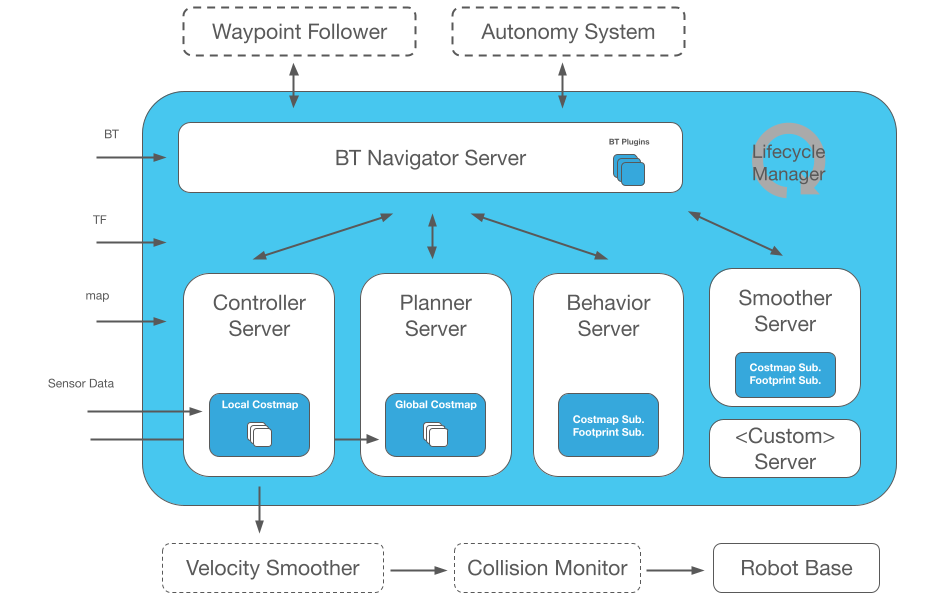
\includegraphics[width=0.8\textwidth]{images/nav2_architecture}
    \caption{Navigation package overview}
    \label{fig:nav2}
\end{figure}

\subsection{Map Server}

This package is used to provide \textbf{map} functionalities to \acrshort{ros}. Basically, it gives you the possibility to \textbf{load} a map from a file and use it for \acrshort{amcl}, or \textbf{save} it after \acrshort{slam} has been run.

\subsection{\acrfull{amcl}}

\acrshort{amcl} is used to \textbf{localize} the robot on a known \textbf{map} using a 2D laser scanner \textbf{probabilistically}. Firstly, once the map is loaded, the initial robot pose \textbf{must be set}\footnote{\acrshort{rviz} lets you set the initial robot pose graphically}: what is going on under the hood is publishing a \code{map} $\rightarrow$ \code{odom} transformation so that the \code{odom} $\rightarrow$ \code{base\_link} one leads to the \textbf{real position} of the robot.

\subsection{\acrfull{slam}}

It is a collection of techniques used to \textbf{localize} and \textbf{map} the environment \textbf{simultaneously}, using 2D laser scans \cite{slam}. Once the map is completely built, it is possible to save it to a file and pass it to the Map Server.

\subsection{Recoveries Server}

It is responsible for executing simple controlled robot movements, like backing up, rotating and stopping when \textbf{recovery} is needed, like when the robot \textbf{hits} something.

\subsection{\acrfull{btnav}}

This one makes use of \textbf{behavior trees} to define the actions to be performed when the robot is in a certain \textbf{state}: for example, when no problem has met, it will continue to navigate and reach the current goal, but when it hits something, the behavior tree will execute the recovery action.

\begin{figure}[h]
    \centering
    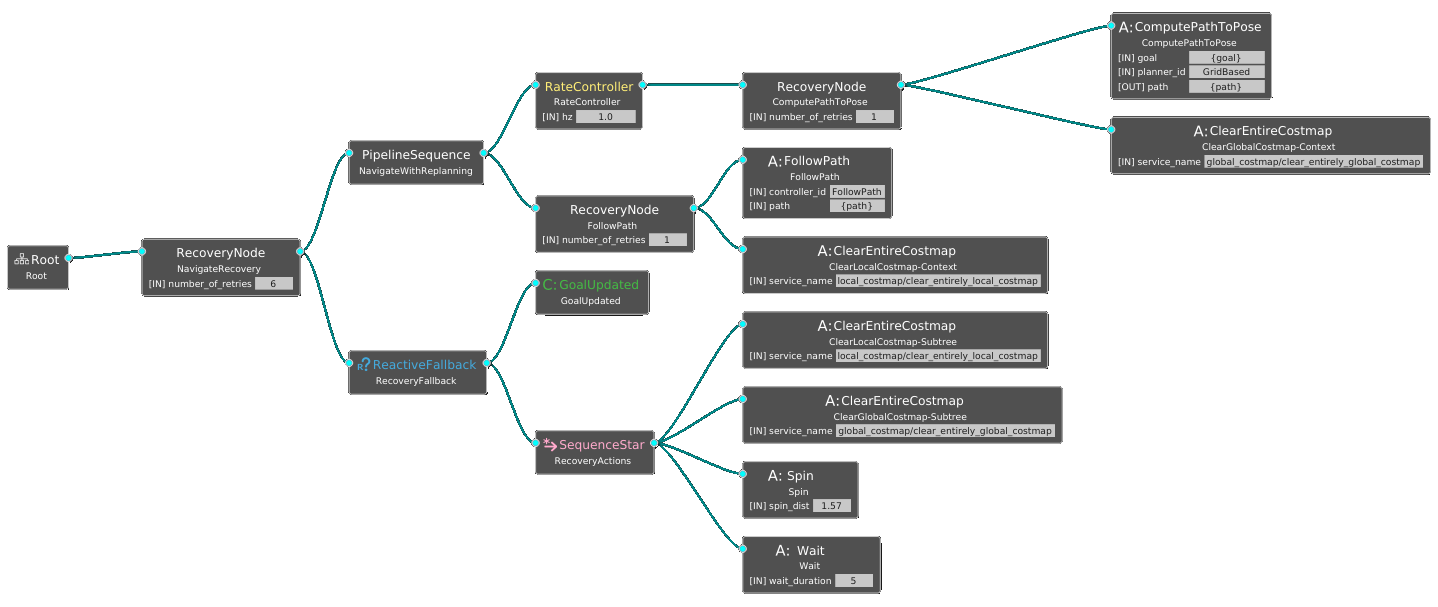
\includegraphics[width=0.9\textwidth]{images/bt-alpha.png}
    \caption{Currently used behavior tree. Groot lets you visualize it, also in real-time. \cite{groot}}
\end{figure}

\subsection{Planner Server}

It implements behavior trees to \textbf{compute path to pose}; it is also possible to choose which pathfinding algorithm you want to use.

\subsection{Controller Server}

It generates \textbf{command velocities} for the wheels using computed path from Planner Server and send them to the robot.

% \subsection{Waypoint Follower} 

% Instead of just setting a single goal, it is possible to navigate a list of waypoints the robot has to pass through. When a waypoint is reached, some plugins can be attached in order to make the robot take a photo, wait for external command or simply wait. Currently, this feature has not been used in the project, because even if multiple rooms are requested to be visited, the planner will only generate subsequent tasks, passing them one by one, after the previous one has been completed.

\subsection{Lifecycle Manager}

All the previous nodes interface with \textbf{Lifecycle Manager}, which brings \acrshort{ros}2 \textbf{managed nodes}\footnote{\textit{A managed life cycle for nodes allows greater control over the state of ROS system. [...] a managed node presents a known interface, executes according to a known life cycle state machine, and otherwise can be considered a black box.} \cite{lifecycle}} concept to the navigation stack: in such a manner, before nodes begin their execution, it \textbf{checks} if all of them were \textbf{launched correctly} and are ready to start, to avoid unexpected behaviors.

\begin{figure}[h]
    \centering
    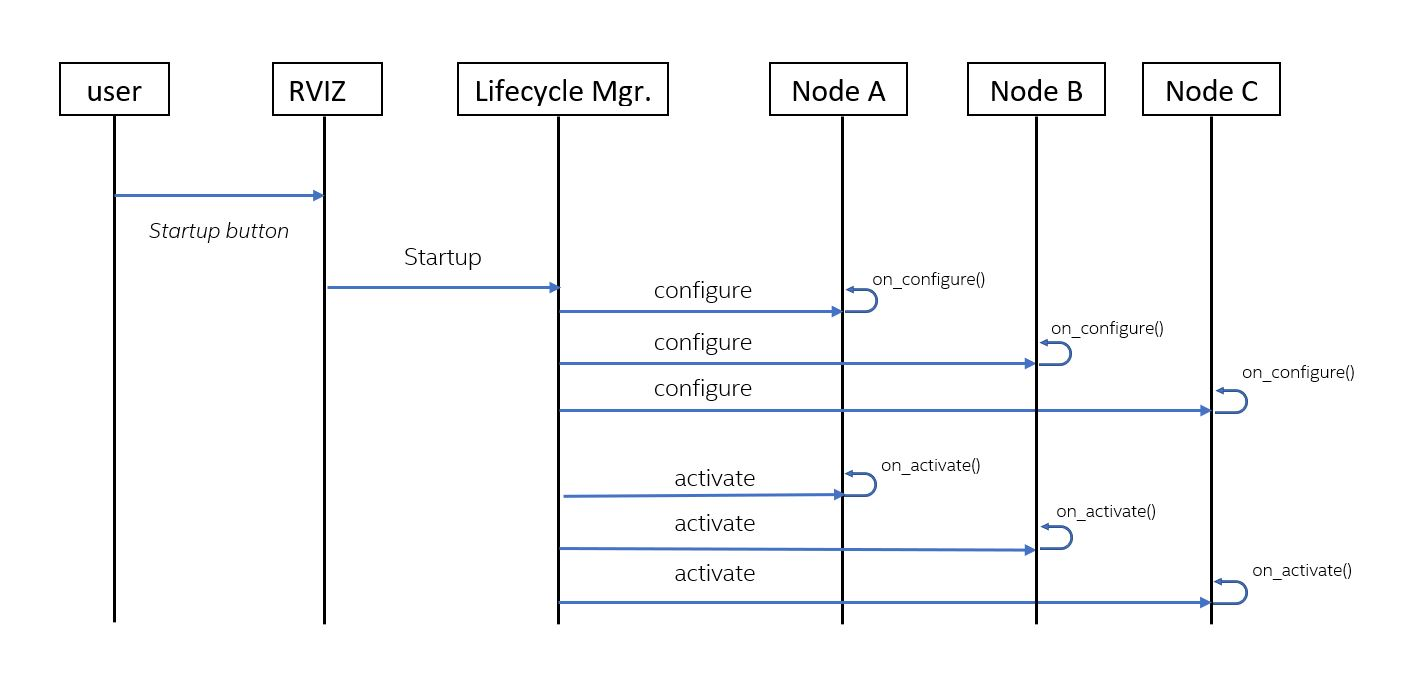
\includegraphics[width=0.8\textwidth]{images/uml_lifecycle_manager}
    \caption{Sequence of service calls when startup is requested}
\end{figure}

\section{Navigation setup}

\begin{wrapfigure}[15]{r}{0.35\textwidth}
    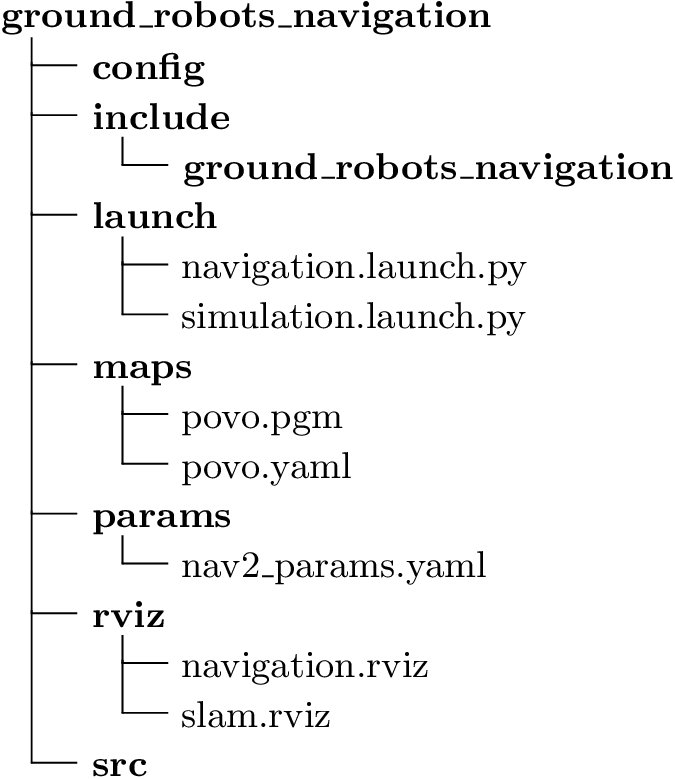
\includegraphics[width=0.35\textwidth]{images/nav_folder}
    \caption{Navigation folder}
\end{wrapfigure}

% sistemare altezza lidar? 0.45 invece di 0.41 come su shelfino (?)

Regardless if the robot is real or simulated, there are always a \code{scan}, \code{odom} and \code{cmd\_vel} topic and a \code{map}, \code{odom} and \code{base\_link}\footnote{All the other links of the robot are connected to the last one, the root one} frame. What is still missing is a way to pass this information to \acrshort{nav2}.

When comes to set navigation properties, the most important is \code{costmap}, which splits into a global and a local one. Here follows a short description:
\begin{itemize}
    \item \textbf{Global}: it is created on the basis of the map provided, saved from \acrshort{slam}, to create the \textbf{general zones} where the robot can and cannot move; it also contains information about how much distance the robot should keep \textbf{from the walls}; used for planning paths.
    \item \textbf{Local}: it makes use of the lidar data to create the \textbf{actual zones} where the robot can and cannot move; in this case, the data coming is dynamic, and it is used to adapt the robot's behavior to changes in the environment (e.g. not expected obstacles, performing \textbf{obstacle avoidance}).
\end{itemize}

In order to automatically visualize robot on the environment on \acrshort{rviz}, a configuration file has been created: it keeps track of the map, the costmaps, the robot shape (described in the \acrshort{urdf} file as discussed in \autoref{sub:robot}), the lidar and the odom frame. 

The map currently used has been created using \acrshort{slam}, and since it is no more possible to control the robot graphically with \acrshort{rviz}, another way has to be found: the solution is the \code{joy} driver package, that makes an \textbf{Xbox controller} capable of setting wheels velocity over \code{cmd\_vel} topic using \textbf{Bluetooth}.

Everything is then put together inside a \textbf{launch file}, which is a custom Python script; on its inside are described what \textbf{nodes} should be started, and also \textbf{parameters} that could be passed from command line(overriding their default value). For example, if you want to start a simulation, you have to set \code{use\_simulator} parameter to \textit{true} (normally it is \textit{false}); the same goes for \textbf{disabling} the \acrfull{gui} of Gazebo\footnote{Simulator}: you can set \textbf{headless} to \textit{true}. These parameters, as just shown, can be used to perform \textbf{conditional checks}, in order to decide whether a node should be started or not.